\documentclass[10pt,a4paper]{article}

\usepackage[utf8]{inputenc}
\usepackage[T1]{fontenc}
\usepackage[spanish,es-nodecimaldot,es-noquoting]{babel}
\usepackage[margin=2cm,top=2.4cm,bottom=2cm]{geometry}
\usepackage{graphicx}
\usepackage{booktabs}
\usepackage{float}
\usepackage{enumitem}
\usepackage{fancyhdr}
\usepackage{caption}

\captionsetup{font=small,labelfont=bf}
\setlist[itemize]{leftmargin=1.2em,itemsep=2pt,topsep=3pt,parsep=0pt}
\setlength{\parskip}{3pt}
\setlength{\parindent}{0pt}

\pagestyle{fancy}
\fancyhf{}
\fancyhead[L]{\footnotesize CC3084 -- Data Science --- Laboratorio 4: Análisis de datos geoespaciales}
\fancyhead[R]{\footnotesize UVG -- Semestre II, 2026}
\fancyfoot[C]{\thepage}
\renewcommand{\headrulewidth}{0.4pt}

\begin{document}

\begin{center}
{\LARGE\bfseries Monitoreo satelital de cianobacterias en los lagos\\[2pt]
de Atitlán y Amatitlán}\\[6pt]
{\normalsize Laboratorio 4 -- CC3084 Data Science -- Sección 20 -- Grupo \#7}\\[4pt]
{\small Marco Carbajal (23025) \quad Carlos Angel (23010) \quad Diego Monroy (23318)}
\end{center}

\vspace{2pt}

\section{Qué se midió y cómo}

Las cianobacterias son microorganismos que, cuando el agua tiene exceso de nutrientes, temperatura alta y poco
movimiento, se multiplican hasta formar floraciones que pueden ser tóxicas. Medirlas con muestreos en campo es caro
y solo describe el punto donde se tomó la muestra, así que en este trabajo se usó observación satelital, que cubre
el lago completo y permite comparar fechas distintas con el mismo criterio.

\begin{itemize}
  \item \textbf{Datos:} 22 imágenes del satélite Sentinel-2 del programa Copernicus, 11 fechas por lago, entre enero
  de 2025 y julio de 2026. Son las fechas oficiales del laboratorio, todas con nubosidad baja.
  \item \textbf{Índice de cianobacteria (NDCI):} compara la luz que el agua refleja en el borde rojo y en el rojo,
  dos colores en los que la clorofila de las cianobacterias deja una huella clara. Se calculó con el script público
  de cianobacterias de Sentinel Hub, que además convierte el índice a clorofila-a en microgramos por litro, la
  unidad que se usa en calidad de agua.
  \item \textbf{Índices de apoyo:} el NDWI separa el agua de la tierra y sirve para medir solo dentro del lago, y el
  NDVI describe la vegetación del entorno.
  \item \textbf{Resolución:} cada dato corresponde a un cuadro de 10 por 10 metros de superficie, es decir 100
  metros cuadrados.
  \item \textbf{Umbral de floración:} se considera floración visible un NDCI mayor a 0.2, valor a partir del cual el
  agua ya presenta una carga alta de material fotosintético en suspensión.
\end{itemize}

\begin{figure}[H]
  \centering
  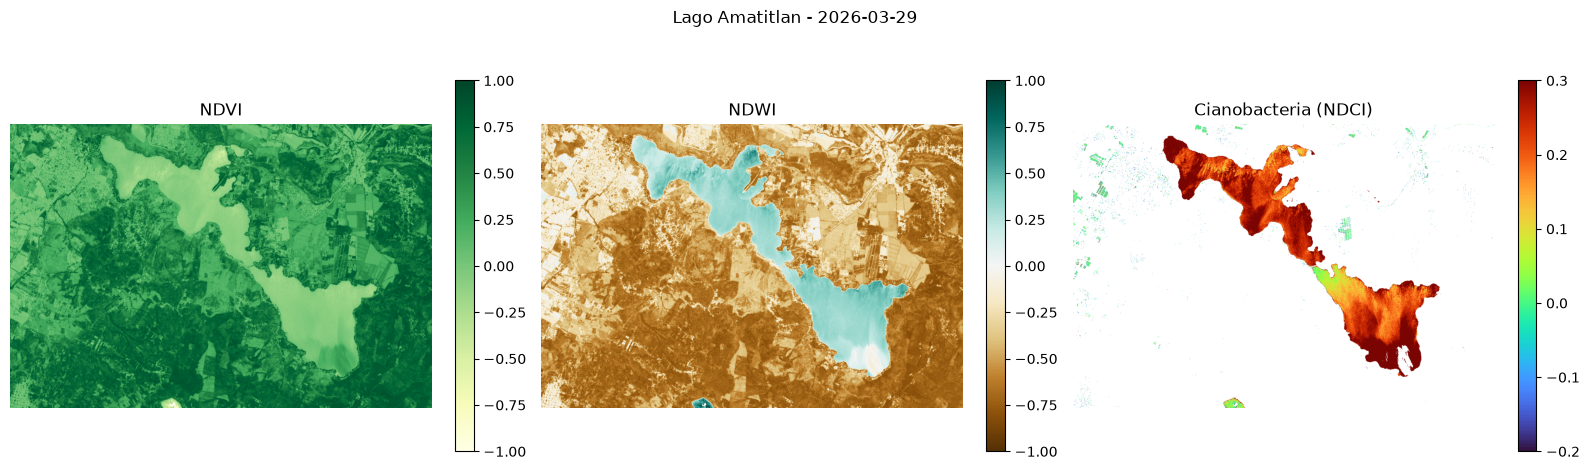
\includegraphics[width=0.95\linewidth]{figuras/indices_amatitlan.png}
  \caption{Los tres índices en el lago de Amatitlán el 29 de marzo de 2026. El NDVI (izquierda) muestra la
  vegetación del entorno, el NDWI (centro) delimita el espejo de agua y el mapa de cianobacteria (derecha) se
  calcula únicamente dentro de esa agua. El rojo indica concentraciones altas.}
\end{figure}

\section{Estado general de los dos lagos}

Los dos lagos están en situaciones opuestas, y la diferencia no es de matiz sino de un orden de magnitud.

\begin{table}[H]
  \centering
  \small
  \begin{tabular}{lcccccc}
    \toprule
    Lago & NDCI promedio & NDCI máximo & Clorofila-a media & Clorofila-a máxima & Fechas con & Superficie \\
     & & & (ug/L) & (ug/L) & floración & afectada \\
    \midrule
    Atitlán   & $-0.026$ & 0.014 & 3.5  & 4.3  & 0 de 11 & 5\%  \\
    Amatitlán & 0.217    & 0.397 & 12.5 & 54.2 & 5 de 11 & 55\% \\
    \bottomrule
  \end{tabular}
  \caption{Resumen de las 11 fechas de cada lago. La superficie afectada es el porcentaje promedio del espejo de
  agua que supera el umbral de floración.}
\end{table}

Amatitlán presenta valores propios de un lago hipereutrófico, es decir con exceso permanente de nutrientes: su
clorofila-a promedio de 12.5 microgramos por litro triplica a la de Atitlán y en la peor fecha llega a 54.2.
Atitlán se mantiene entre 3 y 4 microgramos por litro en todas las fechas, un nivel de agua limpia, y ninguna de
sus imágenes alcanza el umbral de floración.

\section{Cómo cambió en el tiempo}

\begin{figure}[H]
  \centering
  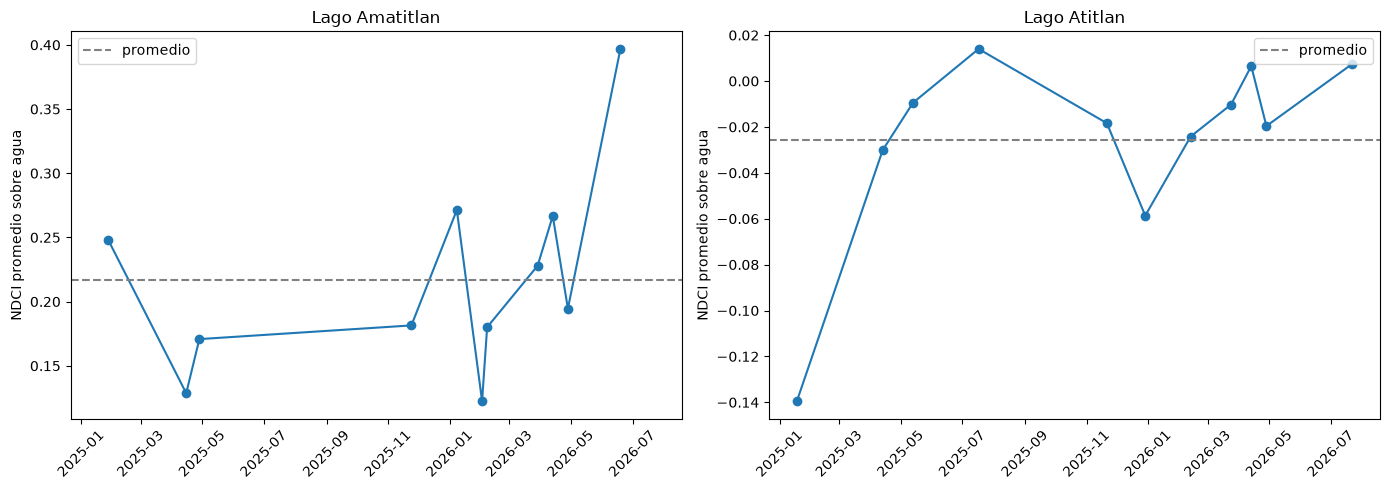
\includegraphics[width=0.95\linewidth]{figuras/serie_temporal.png}
  \caption{Evolución del índice de cianobacteria en cada lago. La línea punteada es el promedio del periodo. Las
  escalas verticales son distintas: el rango completo de Atitlán cabe dentro de las fluctuaciones de Amatitlán.}
\end{figure}

En Amatitlán la serie fluctúa mucho, pero siempre en niveles altos: baja hasta 0.12 en abril de 2025 y febrero de
2026, y sube a 0.27 en enero y abril de 2026. El pico del periodo es el 19 de junio de 2026, con un índice de 0.397
y 54.2 microgramos por litro de clorofila-a, la única fecha que supera el criterio de floración excepcional,
definido como el promedio del lago más una desviación estándar. Es también la única fecha del periodo que cae en
época lluviosa, cuando la escorrentía arrastra nutrientes y el agua está más caliente. Con una sola observación de
esa temporada no se puede afirmar un patrón estacional, pero la dirección coincide con lo esperado. Vale la pena
señalar que el promedio de las fechas de 2026, de 0.24, es mayor que el de 2025, de 0.18.

En Atitlán la serie se mantiene plana alrededor de cero durante los dos años, sin ningún pico. Sus valores más
altos, que aun así son bajos, caen en julio de 2025, abril de 2026 y julio de 2026.

\begin{table}[H]
  \centering
  \small
  \begin{minipage}[t]{0.48\linewidth}
    \centering
    \begin{tabular}{lccc}
      \toprule
      \multicolumn{4}{c}{\textbf{Lago de Atitlán}} \\
      \midrule
      Fecha & NDCI & Clorofila & Superficie \\
            &      & (ug/L)    & afectada \\
      \midrule
      2025-01-18 & $-0.139$ & 0.0 & 24.2\% \\
      2025-04-13 & $-0.030$ & 3.4 & 0.6\%  \\
      2025-05-13 & $-0.009$ & 4.0 & 0.5\%  \\
      2025-07-17 & 0.014    & 4.3 & 1.7\%  \\
      2025-11-21 & $-0.018$ & 4.1 & 12.9\% \\
      2025-12-29 & $-0.059$ & 3.1 & 4.4\%  \\
      2026-02-12 & $-0.024$ & 3.7 & 6.0\%  \\
      2026-03-24 & $-0.010$ & 3.9 & 0.7\%  \\
      2026-04-13 & 0.006    & 4.3 & 0.7\%  \\
      2026-04-28 & $-0.020$ & 3.7 & 0.5\%  \\
      2026-07-22 & 0.007    & 4.2 & 1.0\%  \\
      \bottomrule
    \end{tabular}
  \end{minipage}
  \hfill
  \begin{minipage}[t]{0.48\linewidth}
    \centering
    \begin{tabular}{lccc}
      \toprule
      \multicolumn{4}{c}{\textbf{Lago de Amatitlán}} \\
      \midrule
      Fecha & NDCI & Clorofila & Superficie \\
            &      & (ug/L)    & afectada \\
      \midrule
      2025-01-28 & 0.248 & 11.7 & 76.0\% \\
      2025-04-15 & 0.129 & 5.0  & 28.7\% \\
      2025-04-28 & 0.171 & 5.4  & 42.7\% \\
      2025-11-24 & 0.181 & 6.3  & 37.9\% \\
      2026-01-08 & 0.271 & 14.2 & 81.1\% \\
      2026-02-02 & 0.122 & 5.3  & 14.6\% \\
      2026-02-07 & 0.180 & 6.9  & 41.0\% \\
      2026-03-29 & 0.228 & 9.6  & 68.0\% \\
      2026-04-13 & 0.267 & 13.6 & 88.4\% \\
      2026-04-28 & 0.195 & 5.2  & 41.1\% \\
      2026-06-19 & 0.397 & 54.2 & 87.0\% \\
      \bottomrule
    \end{tabular}
  \end{minipage}
  \caption{Resultados fecha por fecha. La imagen de Atitlán del 18 de enero de 2025 no es comparable con el resto
  por las razones que se explican en la sección de limitaciones.}
\end{table}

\section{Dónde se concentra la floración dentro del lago}

El promedio de un lago esconde lo más útil para el manejo, que es saber dónde ocurre el problema. Al superponer las
11 fechas de Amatitlán aparece un patrón muy estable.

\begin{figure}[H]
  \centering
  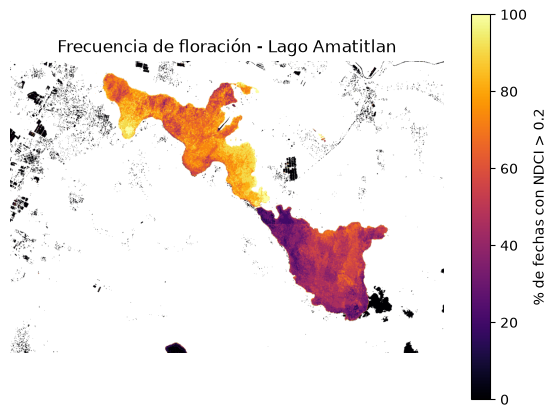
\includegraphics[width=0.56\linewidth]{figuras/frecuencia_amatitlan.png}
  \caption{Porcentaje de las 11 fechas en que cada punto del lago de Amatitlán superó el umbral de floración. La
  cuenca norte, donde desemboca el río Villalobos, aparece en amarillo y naranja; la cuenca sur, del lado de la
  salida hacia el río Michatoya, se mantiene más limpia.}
\end{figure}

Sobre los 14.3 kilómetros cuadrados de agua permanente del lago, la mitad norte promedia un índice de 0.264 y la
mitad sur 0.192. El diez por ciento de los puntos con mayor carga promedia 0.323 y se ubica en la cuenca
norponiente, justo donde entra el río Villalobos con el drenaje del área metropolitana. Esa mitad norte supera el
umbral en cerca del 71 por ciento de las fechas, contra el 44 por ciento de la mitad sur. No se trata de un episodio
aislado sino de una zona de acumulación permanente, y es el sitio donde tendría más sentido concentrar el muestreo
en campo y las alertas al público.

\begin{figure}[H]
  \centering
  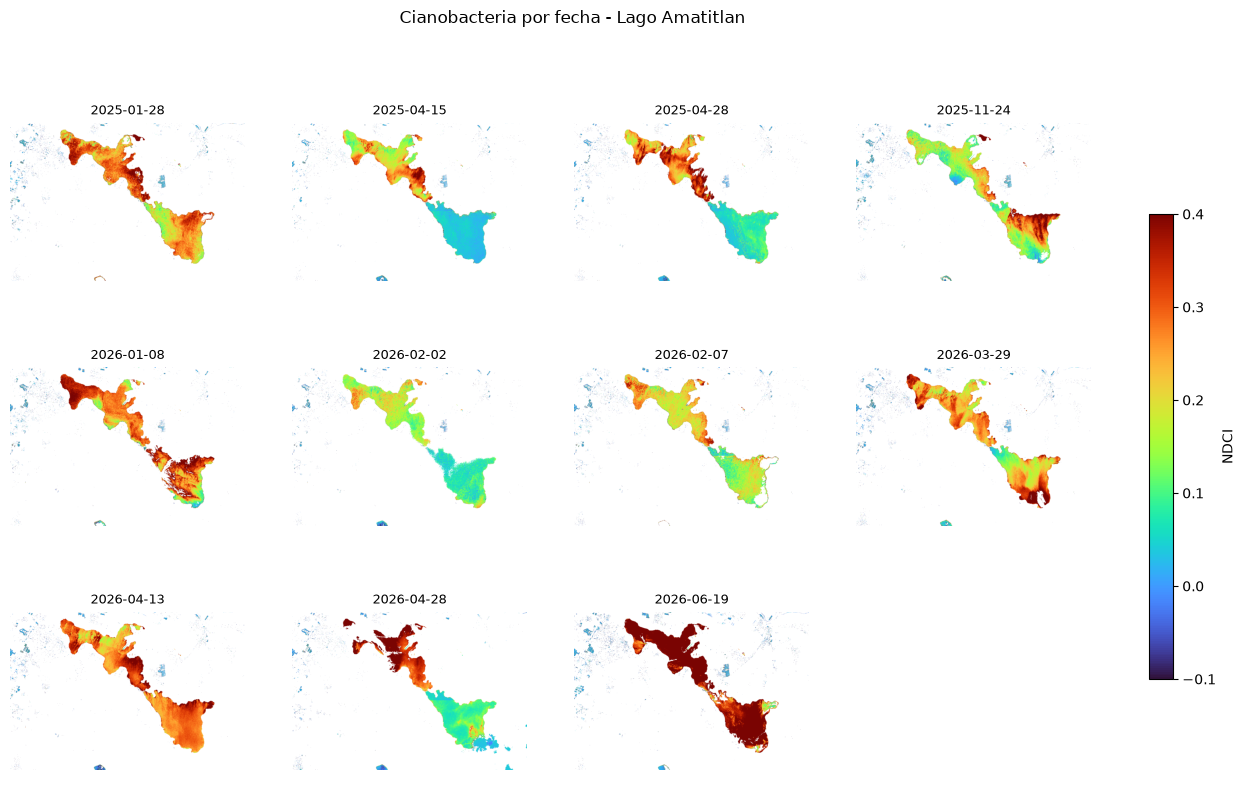
\includegraphics[width=0.92\linewidth]{figuras/rejilla_amatitlan.png}
  \caption{Las 11 fechas del lago de Amatitlán en la misma escala de color. Lo que cambia entre fechas es la
  intensidad, no la ubicación: la cuenca norte siempre aparece más cargada que la sur.}
\end{figure}

En Atitlán no existe ningún patrón equivalente. El promedio de las 11 fechas es plano en todo el espejo de agua y
los puntos más altos y más bajos se ubican prácticamente en el mismo lugar, lo que indica ruido de medición y no una
estructura real. Los únicos valores que superan el umbral forman una franja delgada pegada a la orilla, donde el
cuadro de 10 metros mezcla agua con vegetación ribereña y por eso el índice sube de forma artificial.

\section{Cuánta superficie cubren las floraciones}

\begin{figure}[H]
  \centering
  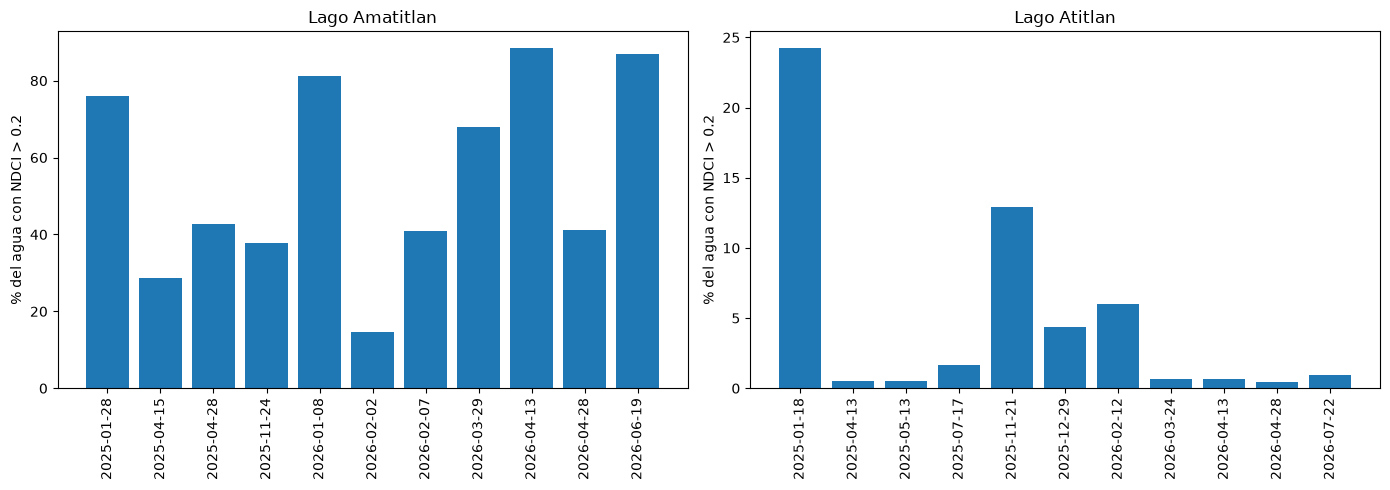
\includegraphics[width=0.95\linewidth]{figuras/extension_floracion.png}
  \caption{Porcentaje del espejo de agua con floración en cada fecha. En Amatitlán, seis de las once fechas superan
  el 40 por ciento del lago. Las escalas verticales son distintas.}
\end{figure}

En Amatitlán la extensión va del 15 por ciento en febrero de 2026 al 88 por ciento en abril de 2026, y en seis de
las once fechas más del 40 por ciento del lago está afectado. La floración de junio de 2026 no es una mancha local:
cubre prácticamente todo el espejo de agua, y el aumento respecto a febrero es positivo en toda la superficie.

En Atitlán los valores parecen altos en cuatro fechas, con 24.2 por ciento en enero de 2025 y 12.9 por ciento en
noviembre de 2025, pero esas cuatro fechas son exactamente las cuatro imágenes con menos píxeles útiles por bruma y
sombra. Son artefactos de la imagen y no floraciones reales, y conviene tenerlo presente porque es el tipo de dato
que puede llevar a una alerta equivocada.

\section{Comparación entre los dos lagos}

\begin{figure}[H]
  \centering
  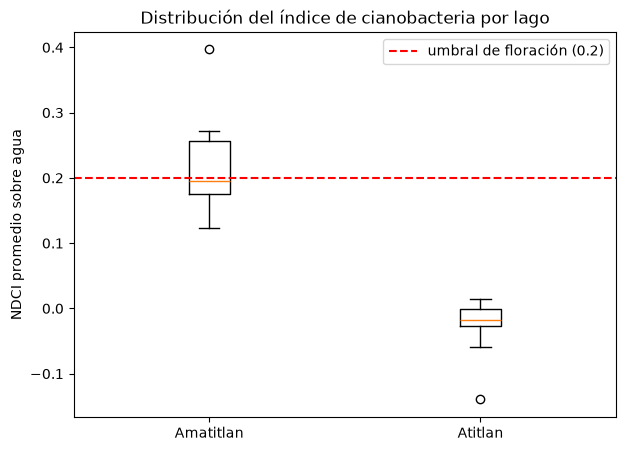
\includegraphics[width=0.45\linewidth]{figuras/boxplot_lagos.png}
  \caption{Distribución del índice en las 11 fechas de cada lago. Las dos distribuciones no se traslapan y solo
  Amatitlán cruza el umbral de floración.}
\end{figure}

\begin{itemize}
  \item \textbf{Intensidad:} Amatitlán promedia 0.217 y llega a 0.397, contra un promedio de $-0.026$ y un máximo de
  0.014 en Atitlán. En clorofila-a la diferencia es de 12.5 frente a 3.5 microgramos por litro en promedio.
  \item \textbf{Frecuencia:} 5 de las 11 fechas de Amatitlán superan el umbral y ninguna de Atitlán lo hace. En
  Amatitlán la floración no es un evento, es un estado permanente que solo cambia de intensidad.
  \item \textbf{Extensión:} 55 por ciento del lago afectado en promedio en Amatitlán, contra 5 por ciento en
  Atitlán, y ese 5 por ciento corresponde a la orilla y a las fechas con bruma.
\end{itemize}

\section{Qué explica la diferencia}

Las causas apuntan a la presión urbana y a la forma misma de cada lago.

\begin{itemize}
  \item \textbf{Carga de nutrientes:} Amatitlán recibe por el río Villalobos el drenaje de la cuenca metropolitana,
  con aguas residuales en su mayoría sin tratamiento, descargas industriales y escorrentía de suelo urbanizado y
  agrícola. Ese aporte entra por la orilla norte, que es precisamente la de mayor carga en los mapas.
  \item \textbf{Volumen y profundidad:} Amatitlán tiene unos 15 kilómetros cuadrados y poca profundidad, mientras
  que Atitlán supera los 100 kilómetros cuadrados y varios cientos de metros de profundidad, de modo que el mismo
  aporte de nutrientes se diluye en un volumen mucho mayor.
  \item \textbf{Temperatura y altitud:} Amatitlán está a menor altitud y su agua es más cálida, condición que
  favorece el crecimiento de las cianobacterias durante todo el año.
  \item \textbf{Uso del suelo:} la cuenca de Atitlán es menos poblada y conserva más bosque y cultivo de café, con
  una presión sobre el agua mucho menor que la del corredor urbano que drena hacia Amatitlán.
\end{itemize}

\section{Limitaciones y confianza en los resultados}

\begin{itemize}
  \item El índice mide clorofila-a, que es un buen indicador de la biomasa de cianobacterias, pero no distingue la
  especie ni mide toxinas. Para decisiones de salud pública sigue siendo necesario el muestreo en campo, aunque
  ahora se sabe dónde y cuándo tomarlo.
  \item La imagen de Atitlán del 18 de enero de 2025 quedó con apenas 17 por ciento de agua útil por las sombras de
  las paredes del cráter con el sol bajo de esa época, y su valor negativo no es comparable con el resto.
  \item Las mediciones de la orilla son menos confiables porque cada cuadro de 10 metros puede mezclar agua con
  vegetación. Esto explica los pocos valores altos que aparecen en Atitlán.
  \item La banda del borde rojo que alimenta el índice de cianobacteria es de 20 metros en origen y se remuestrea a
  10 metros, de modo que el mapa se ve más fino de lo que realmente resuelve esa banda.
  \item Con 11 fechas por lago, y con una sola de ellas en época lluviosa en el caso de Amatitlán, no es posible
  cerrar el análisis estacional. Lo que sí queda demostrado es que en Amatitlán hay floración en todas las fechas,
  incluidas las de época seca.
\end{itemize}

\section{Conclusiones y recomendaciones}

Amatitlán presenta una floración crónica de cianobacterias durante todo el periodo analizado, con una clorofila-a
promedio de 12.5 microgramos por litro, un máximo de 54.2 en junio de 2026 y más de la mitad del lago afectado en
promedio. La floración se concentra siempre en la cuenca norte, del lado del río Villalobos, y el promedio de 2026
es mayor que el de 2025. Atitlán, en cambio, se mantiene estable y limpio en las once fechas, sin ningún evento
detectable.

Con base en estos resultados se recomienda:

\begin{itemize}
  \item Concentrar el monitoreo en campo y las alertas en la cuenca norte de Amatitlán, que es la zona de
  acumulación persistente, y tomar el inicio de la época lluviosa como periodo de vigilancia reforzada.
  \item Sostener el seguimiento satelital como sistema de alerta temprana, ya que cuesta poco, cubre el lago
  completo y permite decidir dónde tomar las muestras en lugar de repartirlas al azar.
  \item Priorizar la reducción de la carga de nutrientes que entra por el río Villalobos, porque los resultados
  espaciales muestran que la floración se origina y se sostiene en ese punto de entrada.
  \item Mantener a Atitlán bajo observación aunque hoy esté limpio, dado que su condición actual depende de un
  volumen de dilución que no lo protege de forma indefinida frente a un aumento de la carga de nutrientes.
\end{itemize}

\end{document}
